\chapter{Diseño}

En este capítulo, nos enfocaremos en el diseño de nuestra plataforma, especificando sus elementos clave, cómo se comunican entre sí y cómo optimizar su funcionamiento para sacar el máximo provecho de sus capacidades. 

También abordaremos la arquitectura general del sistema, el flujo de datos entre los distintos módulos y las decisiones de diseño tomadas para garantizar la escalabilidad, la flexibilidad y la facilidad de uso. 

En adicción se considerarán aspectos relacionados con la experiencia del usuario para asegurar que la plataforma sea lo más intuitiva y eficiente.  

\newpage



\section{Diseño de la arquitectura}

A continuación, se define la arquitectura general de la plataforma, describiendo sus componentes principales y cómo se relacionan entre sí.

La arquitectura se sustenta sobre tres pilares fundamentales:

1. \textbf{Base de datos}: Es la encargada de almacenar la información del usuario, así como otros datos esenciales para el funcionamiento de la aplicación. Se comunica directamente con el backend, enviando y recibiendo información según sea necesario.

2. \textbf{Backend}: Responsable de la lógica y el procesamiento de los datos de la plataforma. En esta capa se encuentra integrado LangChain, el eje principal de este proyecto. El backend se comunica con la base de datos, enviando peticiones y  controlando el flujo de datos. En la capa superior, llamada controlador, se gestiona la comunicación con el frontend, recibiendo solicitudes y transmitiendo los datos necesarios.

3. \textbf{Frontend}: Se encarga de la presentación visual de la aplicación, siendo el medio con el que el usuario interactúa y visualiza la información. Se comunica con el backend para mostrar los datos al usuario y enviar nuevas solicitudes.

\begin{figure}[H]
    \centering
    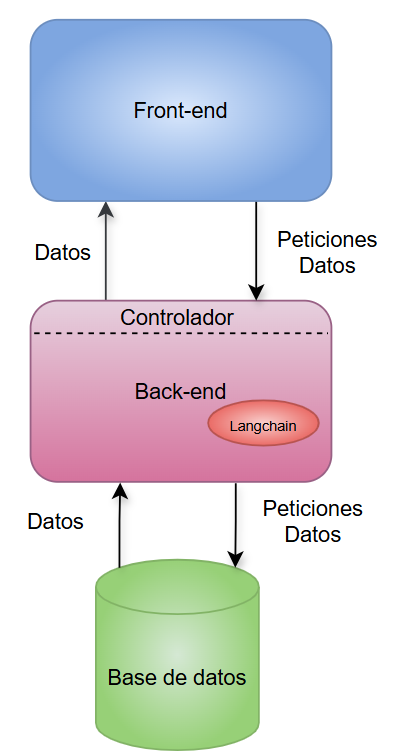
\includegraphics[width=0.5\linewidth]{imagenes/arquitectura.png}
    \caption[\textbf{Representación visual de la arquitectura}]{\textbf{Representación visual de la arquitectura}. En esta imagen se ilustran los elementos clave de la arquitectura, sus interacciones y cómo cada uno de los componentes descritos previamente se conecta y depende entre sí.}
    \label{arquitectura}
\end{figure}



\newpage

\section{Elementos de la arquitectura}

A continuación, se describen detalladamente los distintos elementos que componen la arquitectura de la plataforma.

\subsection{Base de datos}

La base de datos tiene como objetivo almacenar toda la información relevante de los usuarios. Esto incluye tanto datos personales, como nombre de usuario, contraseña o foto de perfil, como información relacionada con su actividad en videojuegos: consolas que posee, componentes de su PC, juegos jugados, títulos que le han gustado o no, suscripciones activas, así como datos proporcionados por APIs externas (por ejemplo, número de horas jugadas) o necesidades especiales que el usuario haya indicado.

Esta información debe almacenarse de forma segura, garantizando tanto la integridad ante posibles pérdidas de datos como la protección de información sensible, especialmente las contraseñas.

Asimismo, la base de datos debe ser capaz de gestionar peticiones de forma rápida y eficiente, permitiendo operaciones de lectura, inserción y modificación de datos sin comprometer el rendimiento del sistema.

En definitiva, la base de datos debe garantizar la disponibilidad, consistencia, flexibilidad y seguridad de la información en todo momento.


\subsection{Backend}

El backend es el núcleo funcional de la plataforma, encargado de procesar la lógica de la aplicación, gestionar los datos de los usuarios y coordinar la comunicación entre el frontend, la base de datos y los modelos de lenguaje.

Una de sus principales responsabilidades es la gestión de usuarios. Para ello, debe mantener un modelo interno que represente al usuario actual, proporcionando métodos que permitan modificar su información, sincronizar los cambios con la base de datos, y manejar correctamente el estado de sesión. Además, debe facilitar el envío y recepción de datos al frontend de manera eficiente y segura.

Otro aspecto central del backend es el sistema de recomendación basado en \texttt{LangChain}. Cuando el usuario realiza una solicitud (por ejemplo, pedir una recomendación de juegos), el backend debe encargarse de preparar el contexto necesario, incluyendo los datos del usuario (si está autenticado), y enviarlo a LangChain. El modelo generará una respuesta personalizada, que luego será procesada y enviada al frontend para su visualización.

En esta capa también se define la configuración de los modelos generativos de lenguajes implicados, cómo interactúan entre sí y cómo se les indica qué tarea deben realizar. Esto incluye desde la selección de cadenas de herramientas hasta el uso de agentes, dependiendo del flujo de la conversación o la consulta del usuario.

El controlador, ubicado en la parte superior del backend, actúa como intermediario entre el frontend y las capas lógicas inferiores. Expone una serie de métodos que permiten al frontend obtener y enviar datos, mientras que las capas inferiores se encargan de realizar operaciones sobre la base de datos y gestionar la lógica de recomendación.

En conjunto, el backend asegura que la plataforma funcione correctamente, manteniendo la coherencia de los datos, ejecutando las operaciones necesarias y respondiendo de forma eficaz a las interacciones del usuario.



\subsection{Frontend}

El frontend es la capa visual de la plataforma y el punto de interacción directa con el usuario. Su diseño debe priorizar la usabilidad, la claridad en la presentación de la información y la adaptación a distintos dispositivos. Para ello, es fundamental distribuir correctamente los elementos en pantalla, emplear una paleta de colores agradable y coherente, y aplicar un diseño responsivo que se adapte a diferentes resoluciones y tamaños de pantalla.

La interfaz contará con una página principal accesible para todos los usuarios, en la que podrán iniciar sesión, registrarse o acceder a una recomendación sencilla sin necesidad de autenticarse. Una vez que el usuario haya iniciado sesión, podrá acceder a funcionalidades más avanzadas, como la edición de su información personal, la solicitud de recomendaciones personalizadas o la consulta de contenido actualizado. Este contenido incluirá noticias destacadas, últimos lanzamientos adaptados a sus consolas y juegos favoritos, o recomendaciones populares entre usuarios con intereses similares.

Desde el punto de vista técnico, el frontend debe comunicarse con el backend mediante peticiones al controlador. A través de estas peticiones podrá recuperar la información necesaria (como recomendaciones o datos del perfil del usuario) y enviar nuevos datos introducidos por el usuario, como actualizaciones de su perfil o nuevas preferencias.

El diseño del frontend no solo debe ser estéticamente atractivo, sino también funcional, guiando al usuario en su experiencia y facilitando la interacción con la plataforma de forma intuitiva y eficiente.


\newpage
\section{Diseño inicial de la interfaz}

Para facilitar el desarrollo de la plataforma, es útil realizar un esbozo preliminar de la interfaz con la que interactuará el usuario. En las siguientes figuras se presentan algunos bocetos que muestran cómo se espera que el usuario visualice y navegue por la plataforma.

\begin{figure}[H]
    \centering
    \fbox{%
        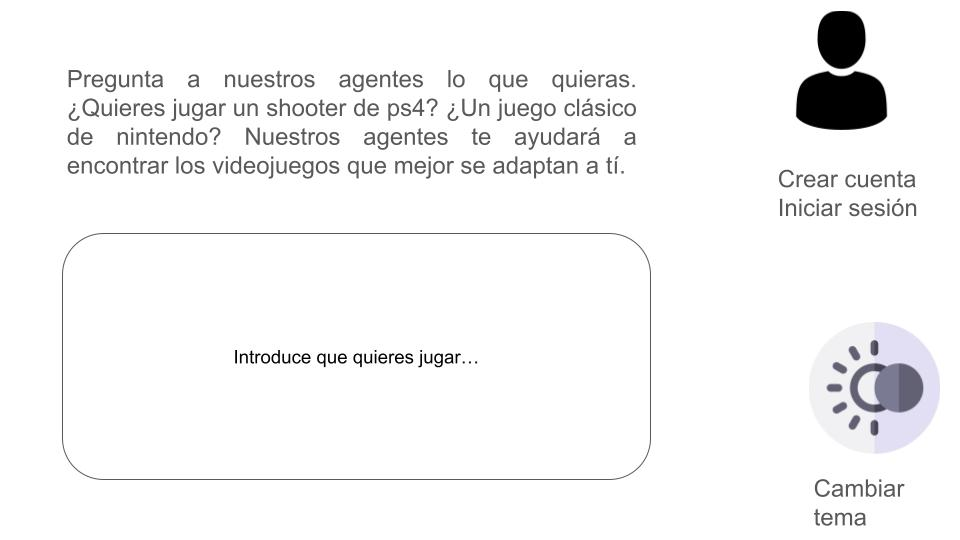
\includegraphics[width=1\linewidth]{imagenes/diPI.jpg}%
    }
    \caption{\textbf{Diseño preliminar de la página de inicio}.}
    \label{fig:pagina-inicio}
\end{figure}

\begin{figure}[H]
    \centering
    \fbox{%
        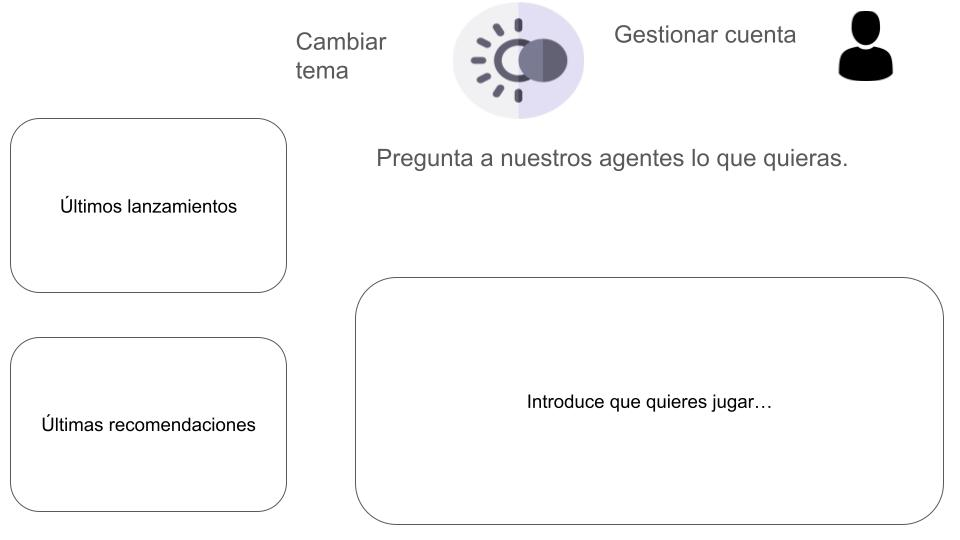
\includegraphics[width=1\linewidth]{imagenes/diPL.jpg}%
    }
    \caption{\textbf{Diseño preliminar de la página principal tras iniciar sesión}.}
    \label{fig:pagina-principal}
\end{figure}

\begin{figure}[H]
    \centering
    \fbox{%
        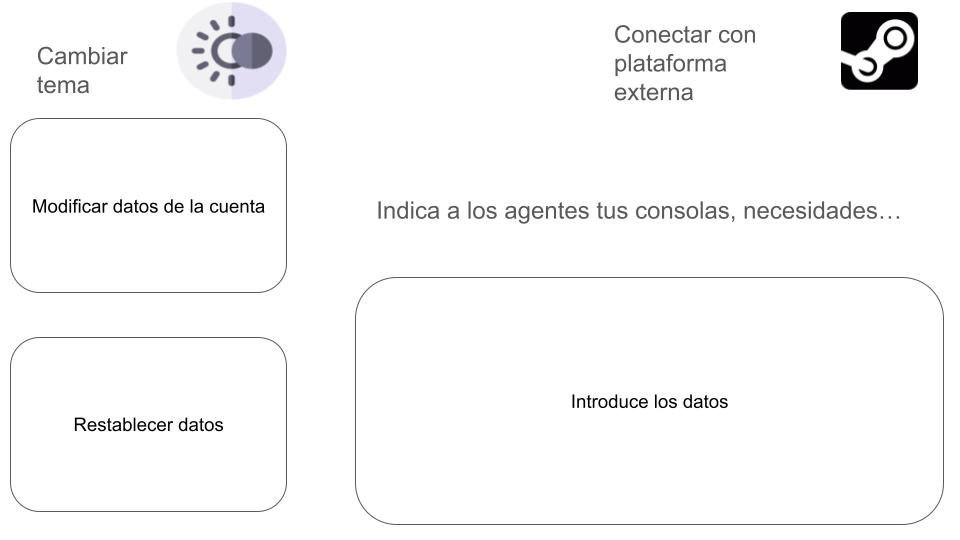
\includegraphics[width=1\linewidth]{imagenes/diA.jpg}%
    }
    \caption{\textbf{Diseño preliminar de la página de ajustes}.}
    \label{fig:pagina-ajustes}
\end{figure}

